\section{Métodos Iterativos}

Um \textbf{método iterativo} é um procedimento matemático que gera uma
sequência de aproximações, e quando esta sequenia é convergente esta
aproximação pode ser aceita como a solução para uma classe de problemas. Um
método iterativo é considerado \textbf{convergente} se a sequência de valores
geradas converge para uma dada aproximação inicial.

Para uma definição mais teórica, o seguinte autor define:

\begin{quotation}

``Um método iterativo consiste em repetir uma determinada operação um certo número
de vezes até que nos seja fornecida uma aproximação, que satisfaça as condições
do problema e, para tal, a sequência de valores deve ser
convergente.''\cite{batista2014metodos}

\end{quotation}

Nos problemas do tipo encontre a raíz da equação, um método iterativo usa
uma suposição inicial para gerar sucessivas aproximações à uma solução. Em
Contraste, \textbf{métodos diretos} tentam resolver o problema em uma sequência
\emph{finita} de operações.

Um método iterativo é formado por quatro partes:~\cite{claudio2000calculo}

\begin{enumerate}[a)]

	\item Estimativa inicial: uma ou mais aproximações para a raiz desejada.

    \item Atualização: uma fórmula que atualize a solução aproximada.

    \item Critério de parada: uma forma de estabelecer quando parar o processo iterativo em qualquer caso.

    \item Estimador de exatidão: está associado ao critério de parada e provê uma estimativa do erro cometido.

\end{enumerate}

	Nas proximas seções serão apresentados as constantes(ou número, arruma
	isso) irracionais utilizando métodos iterativos, bem como a análise de
	convergência do método que está sendo aplicado. A análise de convergência
	foi obtida de forma que é calculado a diferença entre a constate e o valor
	obtido na iteração, ou seja, usamos a medida de erro absoluto. Os
	algoritmos utilizados seguem o mesmo formato no sentido de que sempre que o
	executamos é informado o núemro de maximo de iterações e o erro tolerável,
	quando uma das condições é satisfeita partimso para a análise dos
	resultados obtidos.

\subsection{Número de Ouro}

	O número de ouro, também conhecido como $\phi$, é o resultado da seguinte
	equação:

	\begin{equation}
		x^2-x-1
	\end{equation}

	Existem algums algoritmos para realizar a aproximação neste artigo, sendo
	duas destas formas  abordadas. A primeira utilizando frações continuas e o
	segundo calculando as raizaes da equação utiizando método de newton.

\subsubsection{Frações Continuadas}

	Frações conitinuadas são formas de representar números reais de tal forma
	que a expressão básica tem o seguinte formato:

	\begin{equation}\label{eq:phi}
		a_0 + \frac{b_0}{a_1 + \frac{b_1}{a_n + \dots}}
	\end{equation}

	Para calcular o $\phi$ devemos substituir \emph{a} e \emph{b} por 1. Na
	Fração~\ref{eq:phi}.

	\begin{table}[H]
\centering 
\begin{tabular}{|c|c|c|c|}
\hline 
Iteração & Aproximação &  PHI & Erro \\ 
\hline 
1 & 1.00000000000000 &  1.61803398874989 & 0.61803398874989 \\ 
\hline
2 & 2.00000000000000 &  1.61803398874989 & 0.38196601125011 \\ 
\hline
3 & 1.50000000000000 &  1.61803398874989 & 0.11803398874989 \\ 
\hline
4 & 1.66666666666667 &  1.61803398874989 & 0.04863267791677 \\ 
\hline
5 & 1.60000000000000 &  1.61803398874989 & 0.01803398874989 \\ 
\hline
6 & 1.62500000000000 &  1.61803398874989 & 0.00696601125011 \\ 
\hline
7 & 1.61538461538462 &  1.61803398874989 & 0.00264937336528 \\ 
\hline
8 & 1.61904761904762 &  1.61803398874989 & 0.00101363029772 \\ 
\hline
9 & 1.61764705882353 &  1.61803398874989 & 0.00038692992637 \\ 
\hline
10 & 1.61818181818182 &  1.61803398874989 & 0.00014782943192 \\ 
\hline
\end{tabular}
\label{table:phi-frac}
\caption{Convergência do número de ouro pelo método de frações continuadas}
\end{table}

Como fica ilustrado na tabela, o número já se estabiliza antes mesmo de
chegarmos à 50 iterações.

\begin{figure}[H]
    \centering
    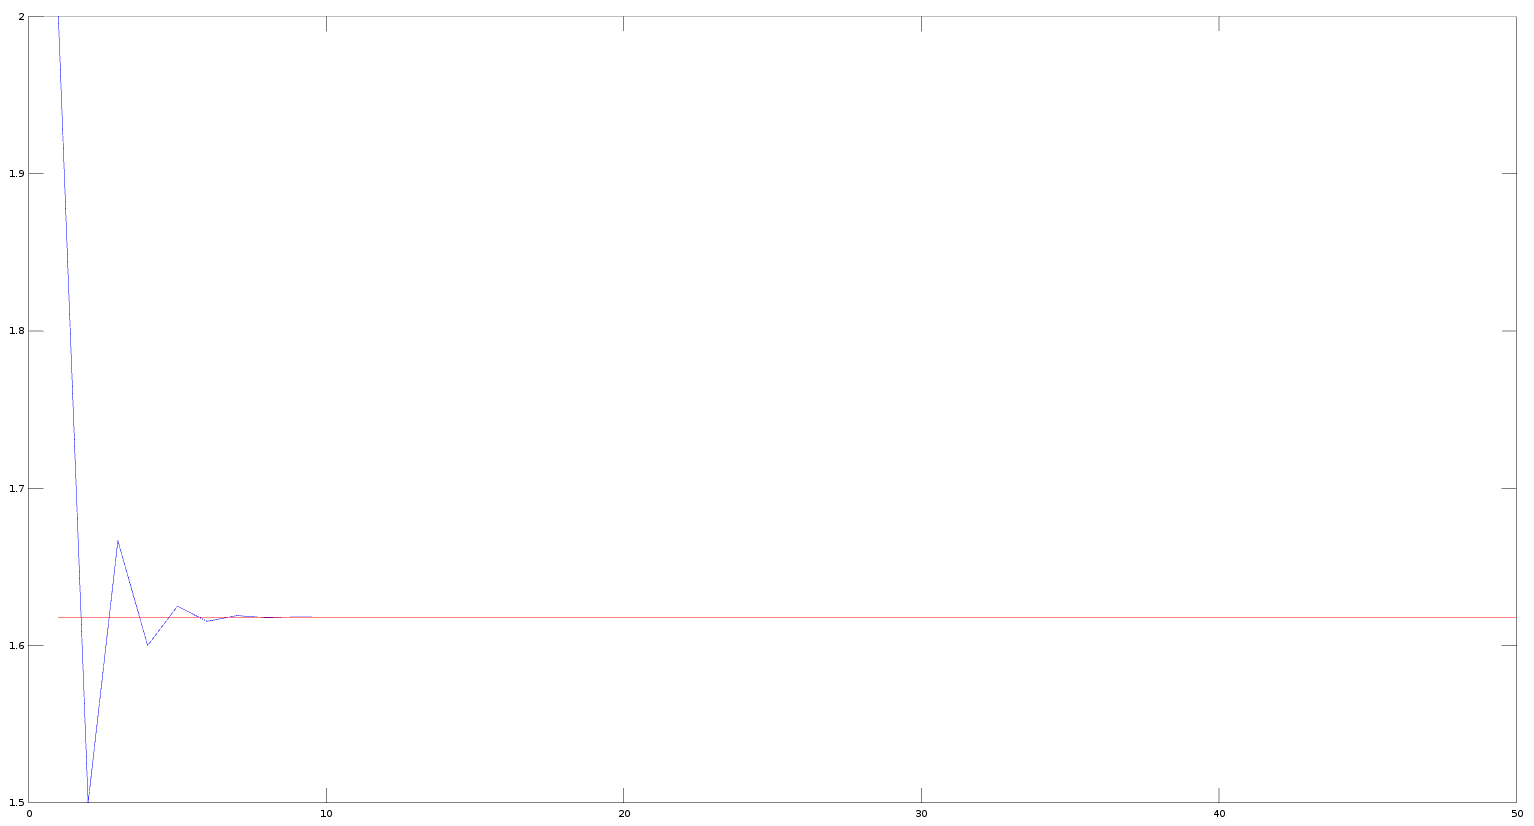
\includegraphics[width=100mm]{golden_frac.png}
    \caption{Convergência do número de ouro pelo método de frações continuadas}
    \label{golden_frac}
\end{figure}


O método iterativo utilizado foi descrito pelo seguinte código:

\begin{lstlisting}

function [x] =  phi_frac(iteration=1)
	aux = 1;
	for i= 1:iteration
		aux = double(1 + 1/aux);
		x(i) = aux;
	end
end

\end{lstlisting}

\subsubsection{Método de Newton}

A ideia do método de Newton é a partir de um valor inicial arbitrário, então a
função é aproximada por sua reta tangente. O $x$ que intercepta a reta e a
função é computado, e ele será uma melhor aproximação que o chute inicial. O
método, então, pode ser iterado.

Analizando novamente o número de ouro, mas com o método de newton, um número
muito menor de iterações é observado.

\begin{table}[H]
\centering 
\begin{tabular}{|c|c|c|c|}
\hline 
Iteração & Aproximação & PHI & Erro \\ 
\hline 
1 & 5.31578947368421e+00 &  1.61803398874989e+00 & 9.00000000000000e+00 \\ 
\hline
2 & 3.03767615760713e+00 &  1.61803398874989e+00 & 2.27811331607708e+00 \\ 
\hline
3 & 2.01512639976464e+00 &  1.61803398874989e+00 & 1.02254975784250e+00 \\ 
\hline
4 & 1.67007003765974e+00 &  1.61803398874989e+00 & 3.45056362104896e-01 \\ 
\hline
5 & 1.61919107776978e+00 &  1.61803398874989e+00 & 5.08789598899588e-02 \\ 
\hline
6 & 1.61803458688502e+00 &  1.61803398874989e+00 & 1.15649088475700e-03 \\ 
\hline
7 & 1.61803398875005e+00 &  1.61803398874989e+00 & 5.98134969331809e-07 \\ 
\hline
8 & 1.61803398874989e+00 &  1.61803398874989e+00 & 1.59872115546023e-13 \\ 
\hline
9 & 1.61803398874989e+00 &  1.61803398874989e+00 & 0.00000000000000e+00 \\ 
\hline
\end{tabular}
\caption{Convergência do número de ouro pelo método de Newton}
\label{table:phi-newton}
\end{table}

Isso pode ser observado no gráfico abaixo.

\begin{figure}[H]
    \centering
    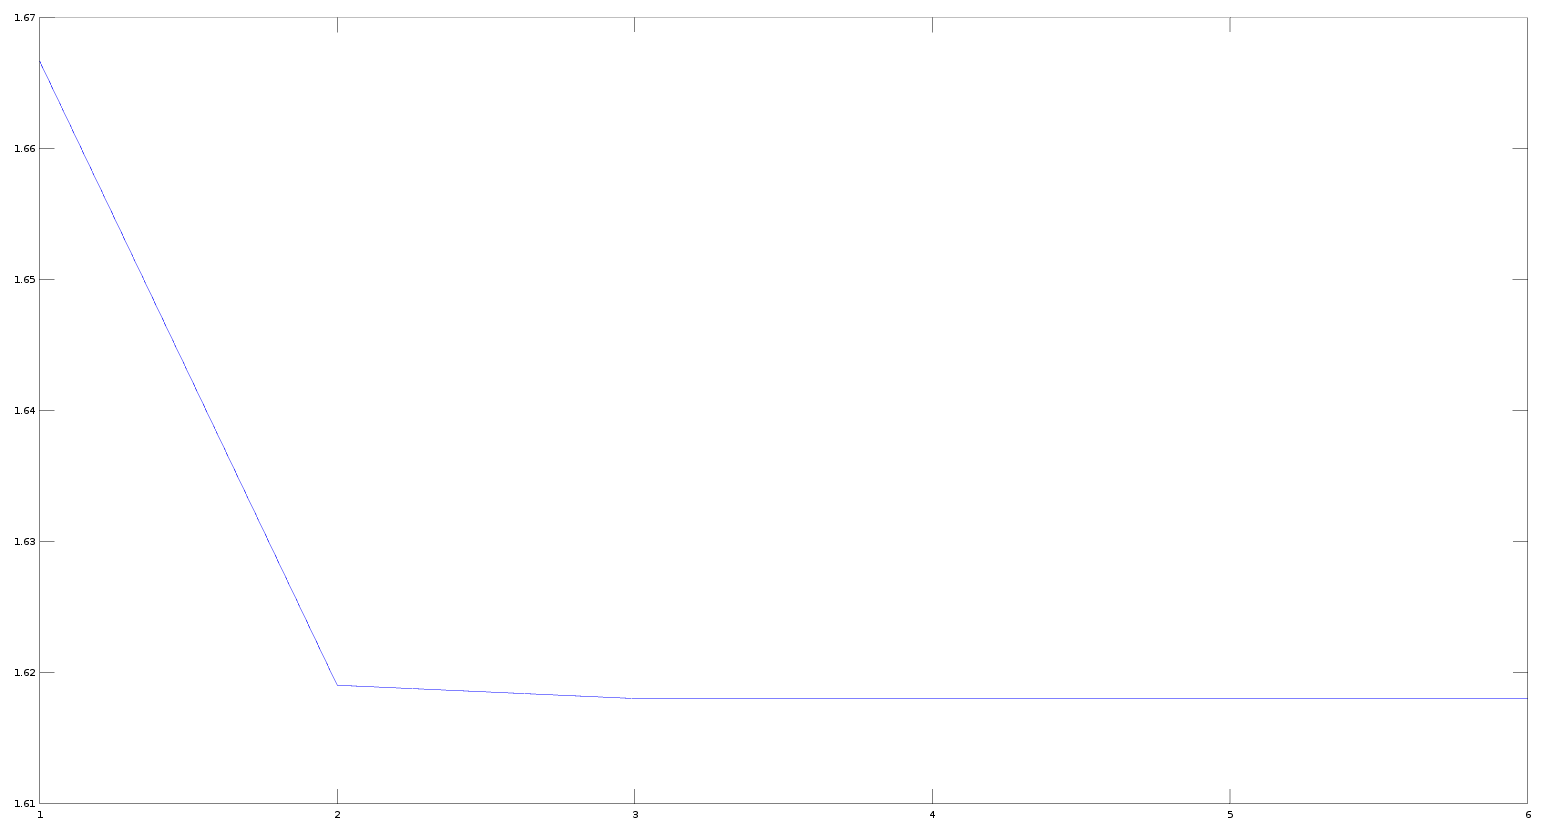
\includegraphics[width=100mm]{golden_newton.png}
    \caption{Convergência do número de ouro pelo método de newton}
    \label{golden_newton}
\end{figure}

O método iterativo utilizado foi descrito pelo seguinte código:

\begin{lstlisting}

function [x, ex] = newton( f, df, x0, tol, nmax)
	f = inline(f);
	df = inline(df);
	x(1) = double(x0 - (f(x0)/df(x0)));
	ex(1) = abs(x(1)-x0);
	k = 2;
	while k <= nmax && ex(k-1) > tol
		 x(k) = double(double(x(k-1)) - double((f(x(k-1))/df(x(k-1)))));
		 ex(k) = abs(x(k)-x(k-1));
		 k = k+1;
	end
end

\end{lstlisting}

\subsection{Pi($\pi$)}

\subsubsection{Método Utilizando Funções Trigonométricas}

Encontramos em um
\href{http://mathforum.org/library/drmath/view/65244.html}{fórum de matemática}
um método iterativo que calcula $ \pi $ de uma forma aparentemente mais simples,
apesar de sua complexidade estar escondida na função \emph{sin}. O método está
descrito a seguir:

\begin{equation}
\label{magic_equation}
P(n+1) = P(n) + sin(P(n))
\end{equation}

$P(n)$ seria a aproximação de $\pi$ na iteração $n$. Esse método consegue
convergir para $\pi$ com um número muito baixo de iterações.

\begin{table}[H]
	\centering
	\begin{tabular}{|c|}
    	\hline
		$P(n)$ \\
		\hline
		3.14112000805986735230135309393517673015594482421875 \\
		\hline
		3.14159265357219563696844488731585443019866943359375 \\
		\hline
		3.14159265358979311599796346854418516159057617187500 \\
		\hline
		3.14159265358979311599796346854418516159057617187500 \\
		\hline
		3.14159265358979311599796346854418516159057617187500 \\
		\hline
		\hline
		$\pi$ \\
		\hline
		3.14159265358979311599796346854418516159057617187500 \\
		\hline
		\hline
		$P(n) - \pi$  Para visualizar a diferença \\
		\hline
		-4.72645529925763696610374609008431434631347656250000 \\
		\hline
		-1.75974790295185812283307313919067382812500000000000 \\
		\hline
		0.00000000000000000000000000000000000000000000000000 \\
		\hline
		0.00000000000000000000000000000000000000000000000000 \\
		\hline
		0.00000000000000000000000000000000000000000000000000 \\
		\hline
	\end{tabular}
	\label{pi_magic}
	\caption{Convergência do $\pi$}
\end{table}

O seguinte gráfico foi gerado com a análise dos resultos:

\begin{figure}[H]
    \centering
    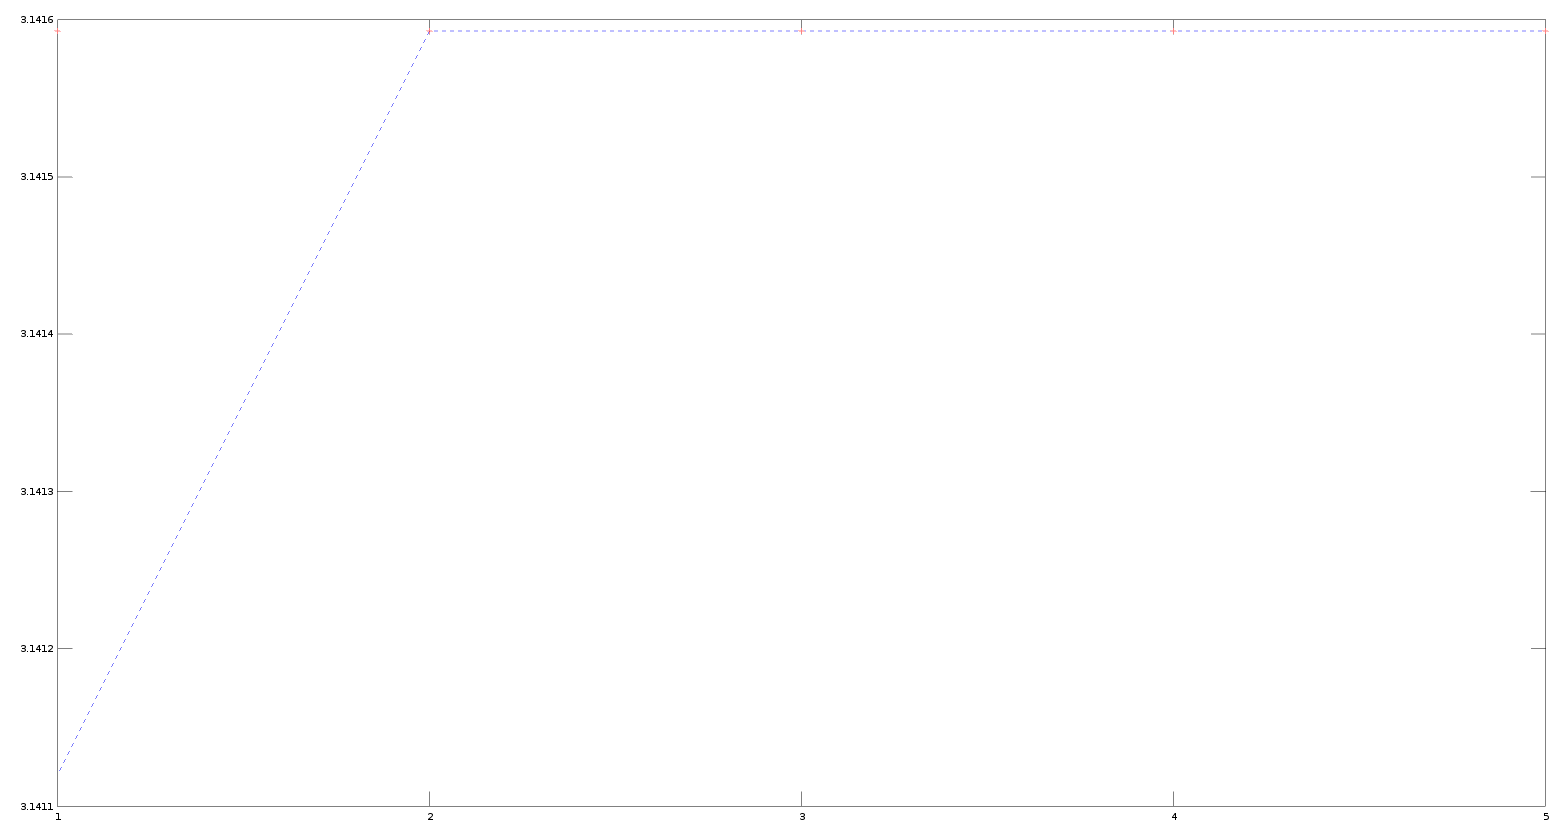
\includegraphics[width=100mm]{pi_magic.png}
    \caption{Convergência do $\pi$}
    \label{fig:pi-magic}
\end{figure}

O método iterativo utilizado foi descrito pelo seguinte código:

\begin{lstlisting}

function [pif, pi_vec] = pi_it(iteration)
	pif(1) = 3 + sin(3);
	pi_vec(1) = pi
	for i = 2:iteration
		pif(i) = pif(i-1) + sin(pif(i-1));
		pi_vec(i) = pi;
		aux = pif(i);
	end
end

\end{lstlisting}

\subsection{$e^x$}

	A função $e^x$ é um função exponencial cuja base é o número de Euler,
	também conhecida como função exponencial natural.

	Para o calculo da da função utilizamos a seguinte série de Taylor
	
	\begin{equation}
		\sum_{n=1}^{n} = \frac{x^n}{n!}
	\end{equation}

	Para exemplificar a foram realizadas 40 iteração para a seguinte função $e^5$, e obtivemos os seguintes resultaodos:

\begin{table}[H]
	\centering
	\begin{tabular}{|c|c|c|c|c|}
    	\hline
		Iteração & Valor Iteração & $e^5$ & Diferença \\
		\hline
		1 & 1.000000 & 148.413159 & 147.413159\\
		\hline
		2 & 6.000000 & 148.413159 & 142.413159\\
		\hline
		3 & 18.500000 & 148.413159 & 129.913159\\
		\hline
		4 & 39.333333 & 148.413159 & 109.079826\\
		\hline
		5 & 65.375000 & 148.413159 & 83.038159\\
		\hline
		6 & 91.416667 & 148.413159 & 56.996492\\
		\hline
		7 & 113.118056 & 148.413159 & 35.295104\\
		\hline
		8 & 128.619048 & 148.413159 & 19.794111\\
		\hline
		9 & 138.307168 & 148.413159 & 10.105991\\
		\hline
		10 & 143.689457 & 148.413159 & 4.723703\\
		\hline
		11 & 146.380601 & 148.413159 & 2.032558\\
		\hline
		12 & 147.603849 & 148.413159 & 0.809311\\
		\hline
		13 & 148.113535 & 148.413159 & 0.299624\\
		\hline
		14 & 148.309568 & 148.413159 & 0.103591\\
		\hline
		15 & 148.379580 & 148.413159 & 0.033579\\
		\hline
		16 & 148.402917 & 148.413159 & 0.010242\\
		\hline
		17 & 148.410210 & 148.413159 & 0.002949\\
		\hline
		18 & 148.412355 & 148.413159 & 0.000804\\
		\hline
		19 & 148.412951 & 148.413159 & 0.000208\\
		\hline
		20 & 148.413108 & 148.413159 & 0.000051\\
		\hline
		21 & 148.413147 & 148.413159 & 0.000012\\
		\hline
		22 & 148.413156 & 148.413159 & 0.000003\\
		\hline
		23 & 148.413159 & 148.413159 & 0.000001\\
		\hline
		24 & 148.413159 & 148.413159 & 0.000000\\
		\hline
		25 & 148.413159 & 148.413159 & 0.000000\\
		\hline
		26 & 148.413159 & 148.413159 & 0.000000\\
		\hline
		27 & 148.413159 & 148.413159 & 0.000000\\
		\hline
		28 & 148.413159 & 148.413159 & 0.000000\\
		\hline
		29 & 148.413159 & 148.413159 & 0.000000\\
		\hline
		30 & 148.413159 & 148.413159 & 0.000000\\
		\hline
		31 & 148.413159 & 148.413159 & 0.000000\\
		\hline
		32 & 148.413159 & 148.413159 & 0.000000\\
		\hline
		33 & 148.413159 & 148.413159 & 0.000000\\
		\hline
		34 & 148.413159 & 148.413159 & 0.000000\\
		\hline
		35 & 148.413159 & 148.413159 & 0.000000\\
		\hline
		36 & 148.413159 & 148.413159 & 0.000000\\
		\hline
		37 & 148.413159 & 148.413159 & 0.000000\\
		\hline
		38 & 148.413159 & 148.413159 & 0.000000\\
		\hline
		39 & 148.413159 & 148.413159 & 0.000000\\
		\hline
		40 & 148.413159 & 148.413159 & 0.000000\\
		\hline
	\end{tabular}
	\label{ex_table}
	\caption{Convergência de $e^5$}
\end{table}

Utilizando a série de Taylor foi percebido que o método converge após 24
iterações.A complexidade deste método encontra-se no cáculo de \emph{n!}.
Podemos observar na Figura~\ref{eq:phi} a representação gráfica da convegência
entre a série e $e^5$. 

\begin{figure}[H] \centering
	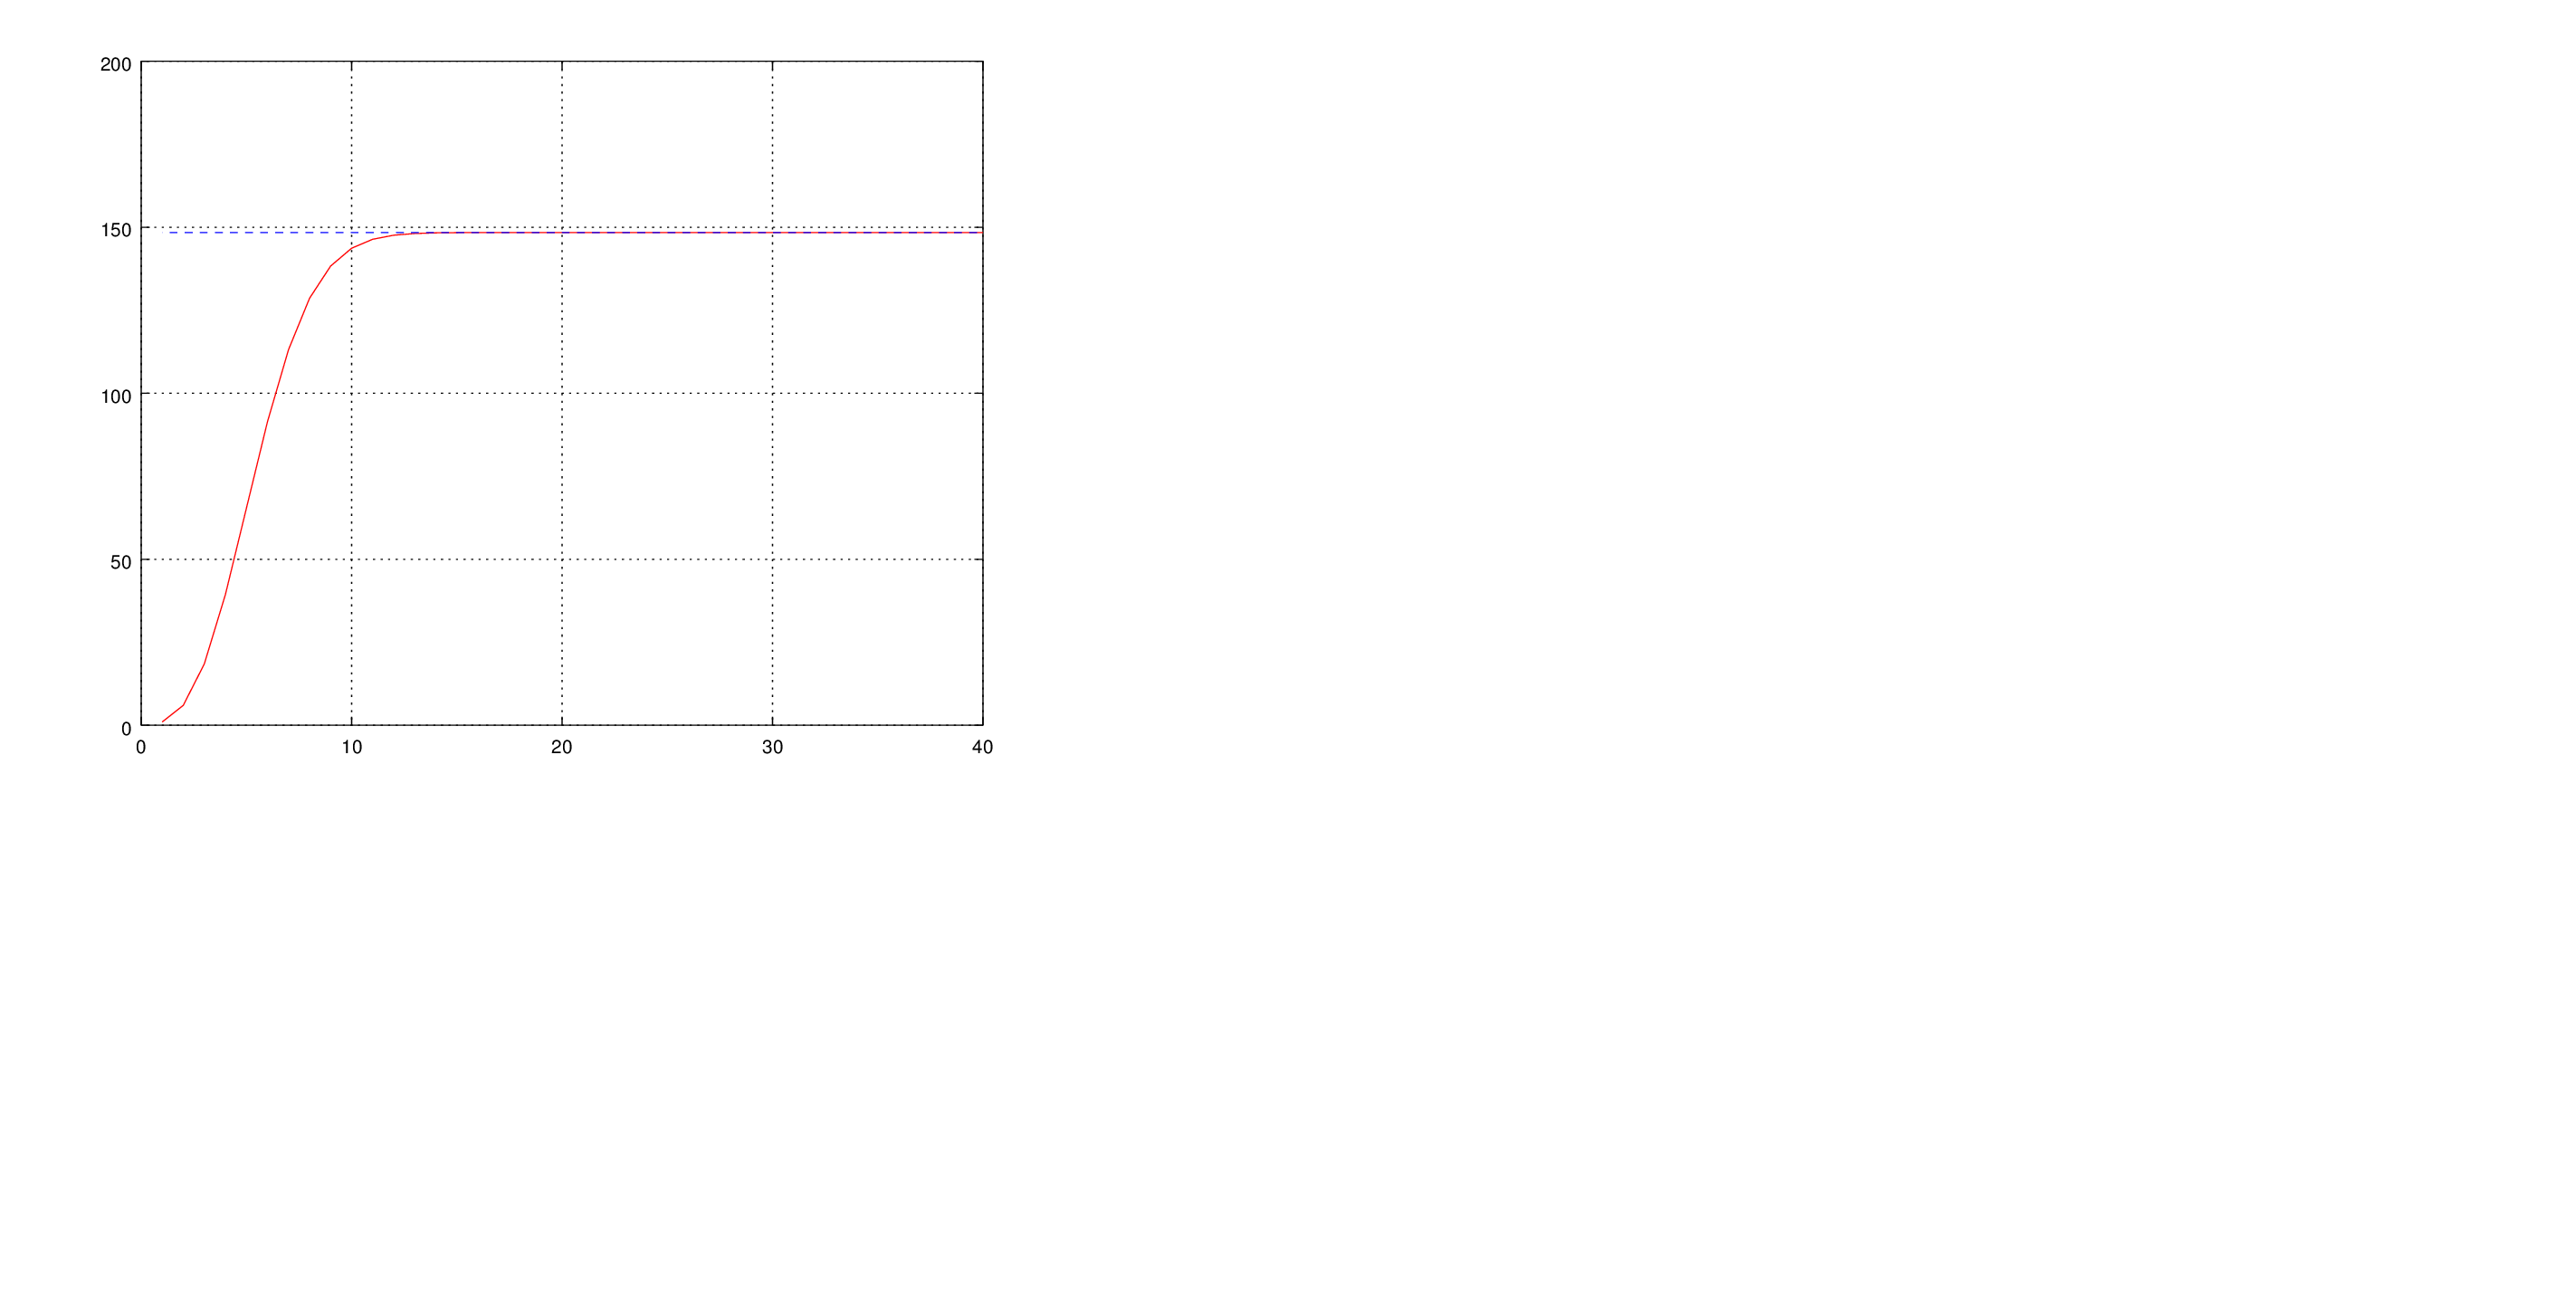
\includegraphics[scale=.75]{ex5.png} 
\caption{Convergência de $e^5$ em 40 iterações}
\label{ex5} 
\end{figure}

Utilizamos o Algoritmo exponential implementado como mostrado a seguir,
que retorna uma matriz de forma que cada coluna representa uma iteração e
a primeira linha o valor calculado, a segunda o valor de $e^5$ e a
tereceira linha é utilizada para guardar a diferença entre $e^5$ o valor
calculado na iteração.

\begin{lstlisting}
function [ex] = exponential(x, iteration)
	ex2 = e^x;
	ex(1,1) = 1;
	ex(2,1) = ex2;
	ex(3,1) = ex2 - ex(1,1);
	for k=2:iteration
		ex(1,k) = ex(1,k-1) + (power(x,k-1) / factorial(k-1));
		ex(2,k) = ex2;
		ex(3,k) = ex2 - ex(1,k);
	end
end
\end{lstlisting}

\subsection{Erdős-Borwein}

A constante de Erdős-Borwein é a soma dos inversos multiplicativos dos números
de Mersenne, e por definição é:

\begin{equation}
	E = \displaystyle\sum_{n=1}^{\infty} \frac{1}{2^n-1} \approx 1.606695152415291763\dots
\end{equation}

Executando no \emph{octave}, obtemos os seguintes resultados:

\begin{table}[H]
	\centering
	\begin{tabular}{|c|c|c|c|}
    	\hline
		Iteração & $E$ & Iteração & $E$ \\
    	\hline
		1 & 1.0000000000 & 19 & 1.6066932451 \\
    	\hline
		2 & 1.3333333333 & 20 & 1.6066941987 \\
    	\hline
		3 & 1.4761904762 & 21 & 1.6066946756 \\
    	\hline
		4 & 1.5428571429 & 22 & 1.6066949140 \\
    	\hline
		5 & 1.5751152074 & 23 & 1.6066950332 \\
    	\hline
		6 & 1.5909882232 & 24 & 1.6066950928 \\
    	\hline
		7 & 1.5988622390 & 25 & 1.6066951226 \\
    	\hline
		8 & 1.6027838076 & 26 & 1.6066951375 \\
    	\hline
		9 & 1.6047407548 & 27 & 1.6066951450 \\
    	\hline
		10 & 1.6057182719 & 28 & 1.6066951487 \\
    	\hline
		11 & 1.6062067917 & 29 & 1.6066951506 \\
    	\hline
		12 & 1.6064509919 & 30 & 1.6066951515 \\
    	\hline
		13 & 1.6065730771 & 31 & 1.6066951519 \\
    	\hline
		14 & 1.6066341160 & 32 & 1.6066951522 \\
    	\hline
		15 & 1.6066646345 & 33 & 1.6066951523 \\
    	\hline
		16 & 1.6066798935 & 34 & 1.6066951524 \\
    	\hline
		17 & 1.6066875230 & 35 & 1.6066951524 \\
    	\hline
		18 & 1.6066913377 & 36 & 1.6066951524 \\
    	\hline
	\end{tabular}
	\label{erdos_table}
	\caption{Convergência do $E$}
\end{table}

Podemos ver o número se estabilizando no seguinte gráfico, construído a partir
dos resultados da tabela.

\begin{figure}[H]
    \centering
    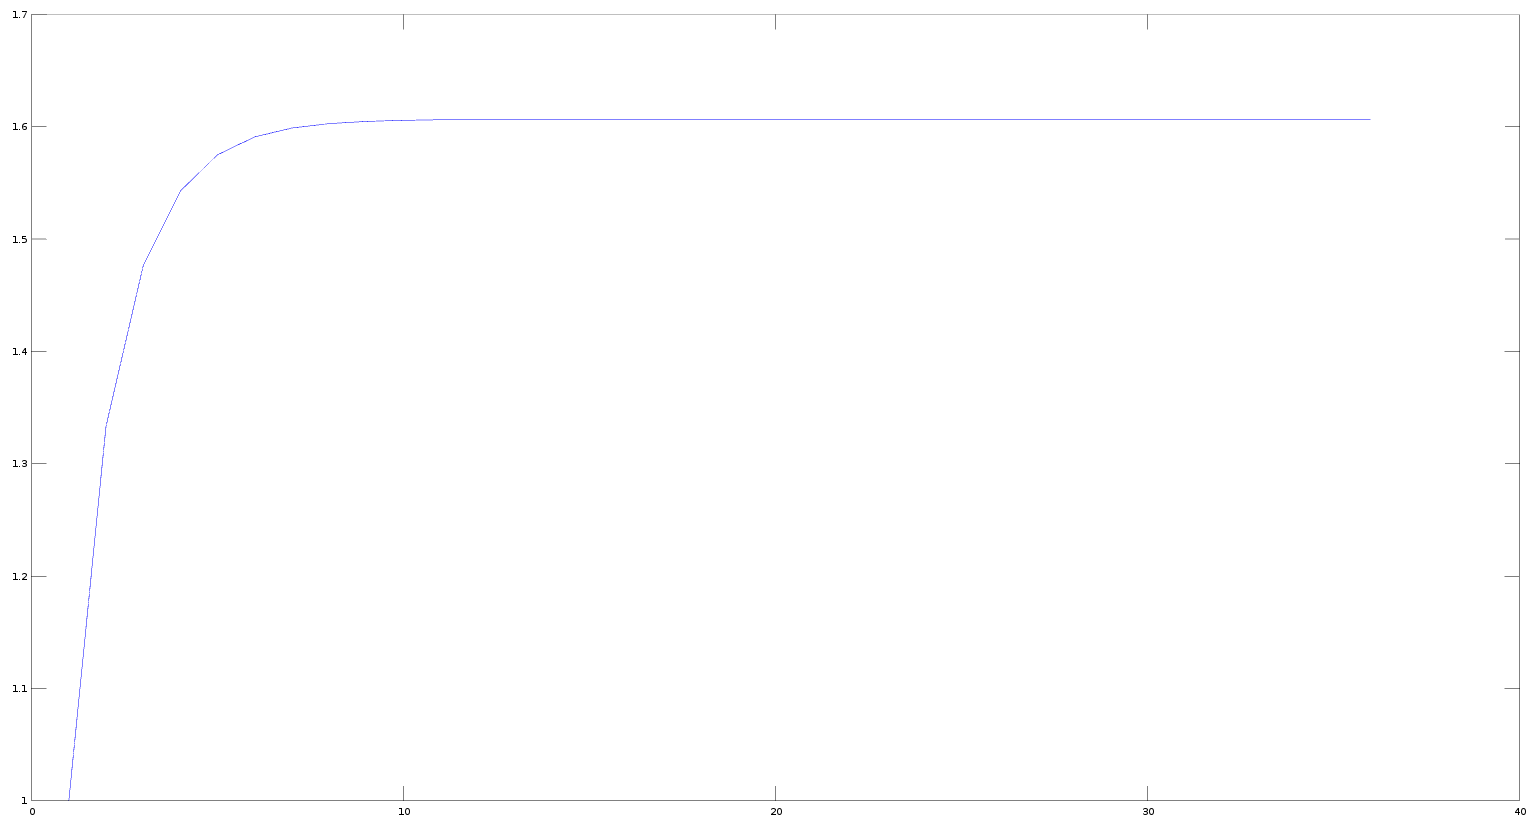
\includegraphics[width=100mm]{erdos.png}
    \caption{Convergência do erdős-borwein em 50 iterações}
	\label{erdos_graphic}
\end{figure}

A definição de $E$ foi codificada da seguinte maneira:

\begin{lstlisting}

function [er] = erdos(iteration)
	er(1) = 1;
	for i=2:iteration
		er(i) = er(i-1) + (1 / ((2^i)-1));
	end
end

\end{lstlisting}
